% !TeX root = ../../main.tex
\subsection{SNORT}

Foi feita a automatização do processo de monitoramento dos alertas do Snort, 
foram criadas regras personalizadas no arquivo \textit{/etc/snort/rules/local.rules}, como mostrado na Figura \ref{fig:snort8}. 
Essas regras foram configuradas para detectar tráfego de rede relacionado a protocolos como ICMP,
 SSH, HTTP e HTTPS. Com essas regras em vigor, o Snort será capaz de identificar e gerar alertas sempre que
  for detectado tráfego suspeito ou malicioso relacionado a esses protocolos, 
  permitindo uma resposta mais rápida e eficaz a potenciais ameaças na rede.    

\begin{figure}[H]
    \centering
    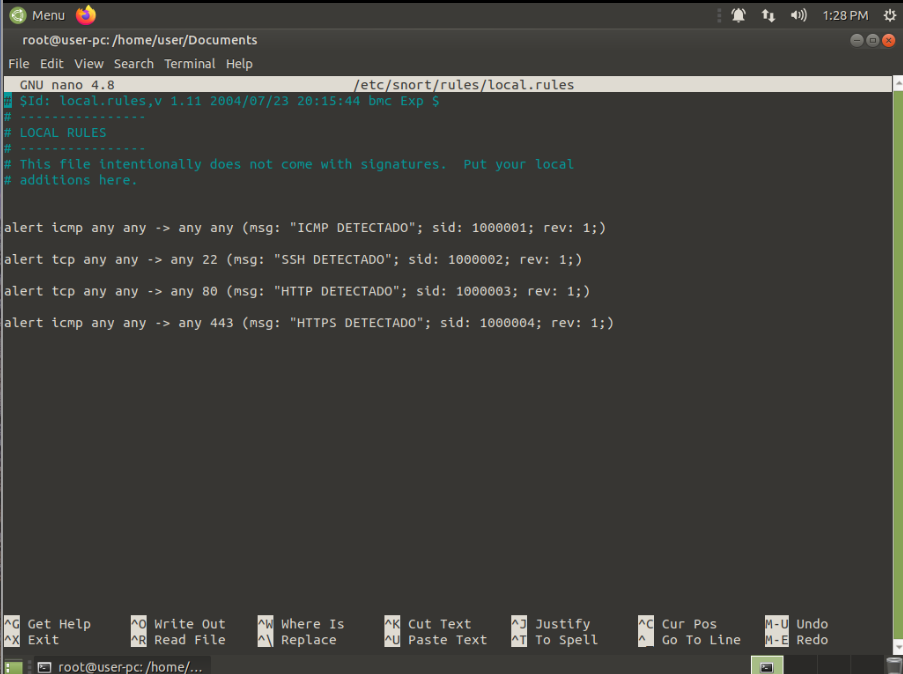
\includegraphics[width=1\linewidth]{fig/snort/snort8.png}
    \caption{Adição de novas regras personalizadas no arquivo local.rules para detectar tráfego ICMP, SSH, HTTP e HTTPS.}
    \label{fig:snort8}
\end{figure}

Na Figura \ref{fig:snort9}, é possível observar a ativação e inicialização do serviço
\textit{snort-monitor} por meio dos comandos \textit{systemctl enable snort-monitor} e
\textit{systemctl start snort-monitor}. Em seguida, o comando \textit{systemctl status snort-monitor}
confirmou que o serviço estava ativo e em execução, indicando que o monitoramento de alertas do Snort
foi configurado corretamente.

\begin{figure}[H]
    \centering
    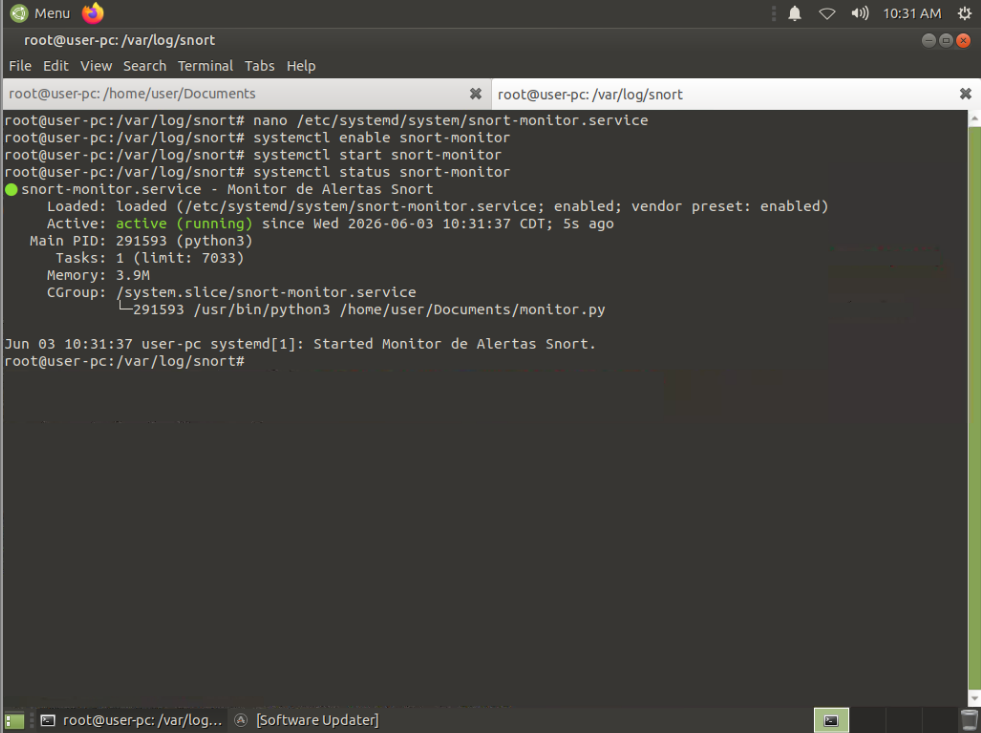
\includegraphics[width=1\linewidth]{fig/snort/snort9.png}
    \caption{Inicialização do serviço snort-monitor;
    1. Comandos para habilitar, iniciar e verificar o status do serviço;
    2. Resultado indicando que o serviço está ativo e em execução}
    \label{fig:snort9}
\end{figure}

Foi criado o arquivo monitor.py \ref{lst:monitor} para monitorar o arquivo de alertas do Snort e 
enviar notificações utilizando o notify-send. O script lê o conteúdo do arquivo de alertas,
 verifica se há novas entradas e envia uma notificação para cada novo alerta detectado.
  O script foi configurado para ser executado periodicamente, garantindo que as notificações 
  sejam enviadas em tempo real sempre que um novo alerta for gerado pelo Snort.

Na Figura \ref{fig:snort10}, foi feita a configuração do script monitor.py para ser executado
utilizando a interface \textit{Startup Program}, que executa o arquivo monitor.py automaticamente
 durante a inicialização do sistema. Dessa forma, 
 o monitoramento dos alertas do Snort e o envio de notificações estarão ativos desde o momento em que o 
 sistema for iniciado, garantindo uma resposta imediata a qualquer evento detectado pelo Snort.

\begin{figure}[H]
    \centering
    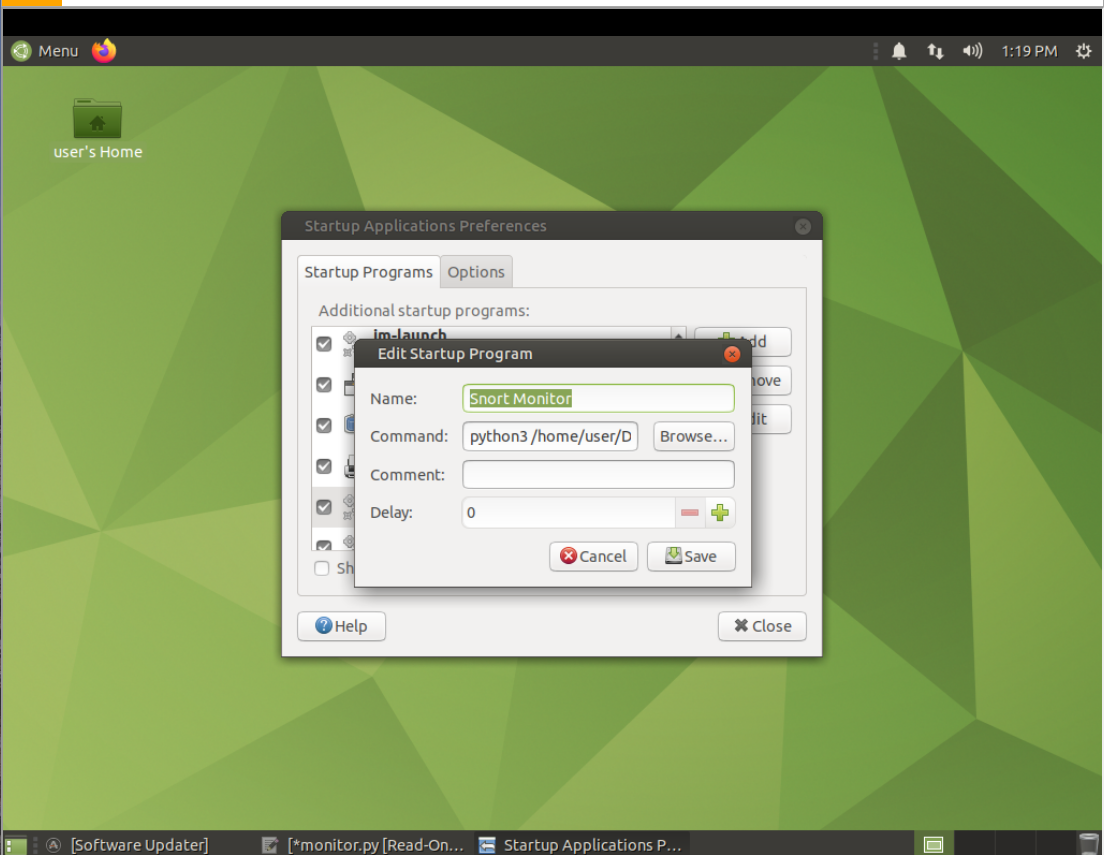
\includegraphics[width=1\linewidth]{fig/snort/snort10.png}
    \caption{Configuração do monitor.py para inicialização automática pelo Startup Program}
    \label{fig:snort10}
\end{figure}

Já na Figura \ref{fig:snort11}, é possível observar o resultado do monitoramento do arquivo de alertas do Snort,
onde cada nova entrada no arquivo de alertas gera uma notificação utilizando o notify-send. As notificações exibem 
o conteúdo dos alertas, permitindo que o usuário seja informado em tempo real.


\begin{figure}[H]
    \centering
    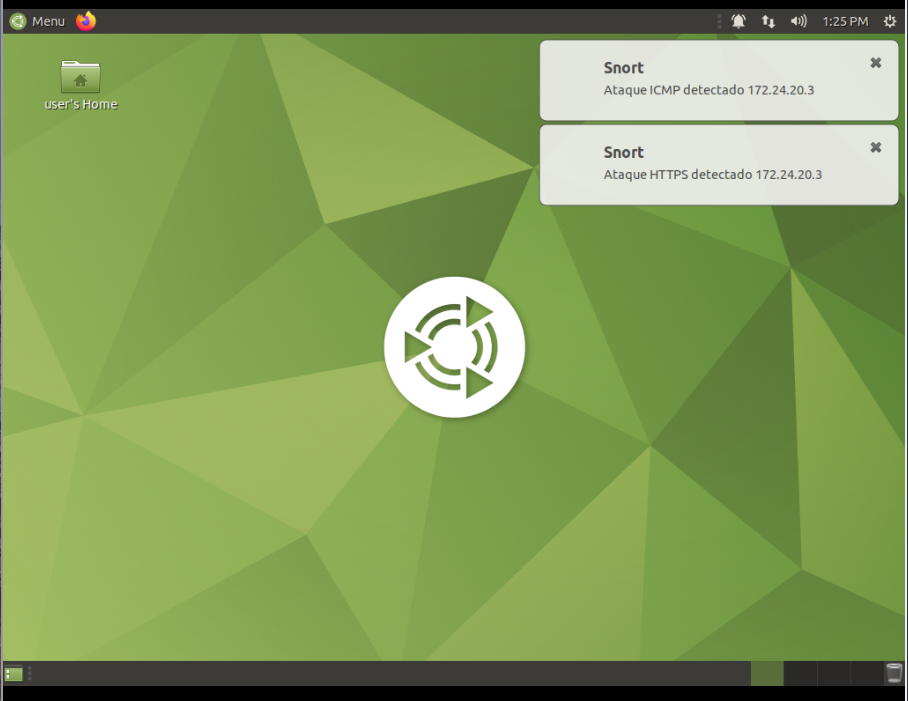
\includegraphics[width=1\linewidth]{fig/snort/snort11.png}
    \caption{Notificações geradas a partir do monitoramento dos alertas do Snort}
    \label{fig:snort11}
\end{figure}
